\documentclass[11pt,letterpaper]{article}

\usepackage[margin=0.7in]{geometry}
\usepackage{graphicx}
\usepackage{booktabs}
\usepackage{array}
\usepackage{parskip}
\usepackage{microtype}
\usepackage[T1]{fontenc}
\usepackage{lmodern}
\usepackage{hyperref}

\title{\textbf{CSE-307 Operating Systems}\\
Learning-Augmented Page Replacement:\\
Classical Algorithms Meet Adaptive Prediction}
\author{Student: Md. Mahdi Israk Mahir \quad Student ID: 202414016\\Track 1}
\date{}

\begin{document}
\maketitle
\thispagestyle{empty}

\section{Problem Framing}
Page replacement decides which resident page should leave memory when a new page is referenced. FIFO and LRU are inexpensive online policies, while Optimal (Belady's) is an offline upper-bound that knows future references. This paper studies whether a small learned policy can use current-state signals to make useful eviction decisions when the access pattern changes after deployment.

\section{Implementation and Learned Component}
The implementation uses four frames and ten possible pages. FIFO maintains arrival order; LRU tracks the most recent reference position; and Optimal evicts the resident page with the farthest next use.

The learned policy is a shallow decision tree trained on a separate synthetic trace. For every resident candidate, it receives only information available at the current miss: page age, access frequency, recency rank, and page identifier. Training labels identify the candidate that Optimal would evict on the training trace. Future references are never supplied as runtime features.

\section{Experimental Setup}
The evaluation trace contains 800 references and is generated with a fixed seed (307). The first 400 references are locality-heavy: pages 0--4 are favored and occasional sequential accesses are inserted. The second 400 references switch to a random/bursty pattern over pages 0--9. Each policy is evaluated separately in both phases using page-fault count and hit ratio.

\section{Results}

\begin{table}[h]
\centering
\caption{Page-replacement results before and after the workload shift.}
\begin{tabular}{lrrrr}
\toprule
\textbf{Policy} & \textbf{Locality faults} & \textbf{Locality hit} & \textbf{Shift faults} & \textbf{Shift hit}\\
\midrule
FIFO    & 81 & 79.8\% & 188 & 53.0\%\\
LRU     & 64 & 84.0\% & 185 & 53.8\%\\
Optimal  & 40 & 90.0\% & 119 & 70.3\%\\
Learned & 54 & 86.5\% & 223 & 44.3\%\\
\bottomrule
\end{tabular}
\end{table}

\begin{figure}[h]
\centering
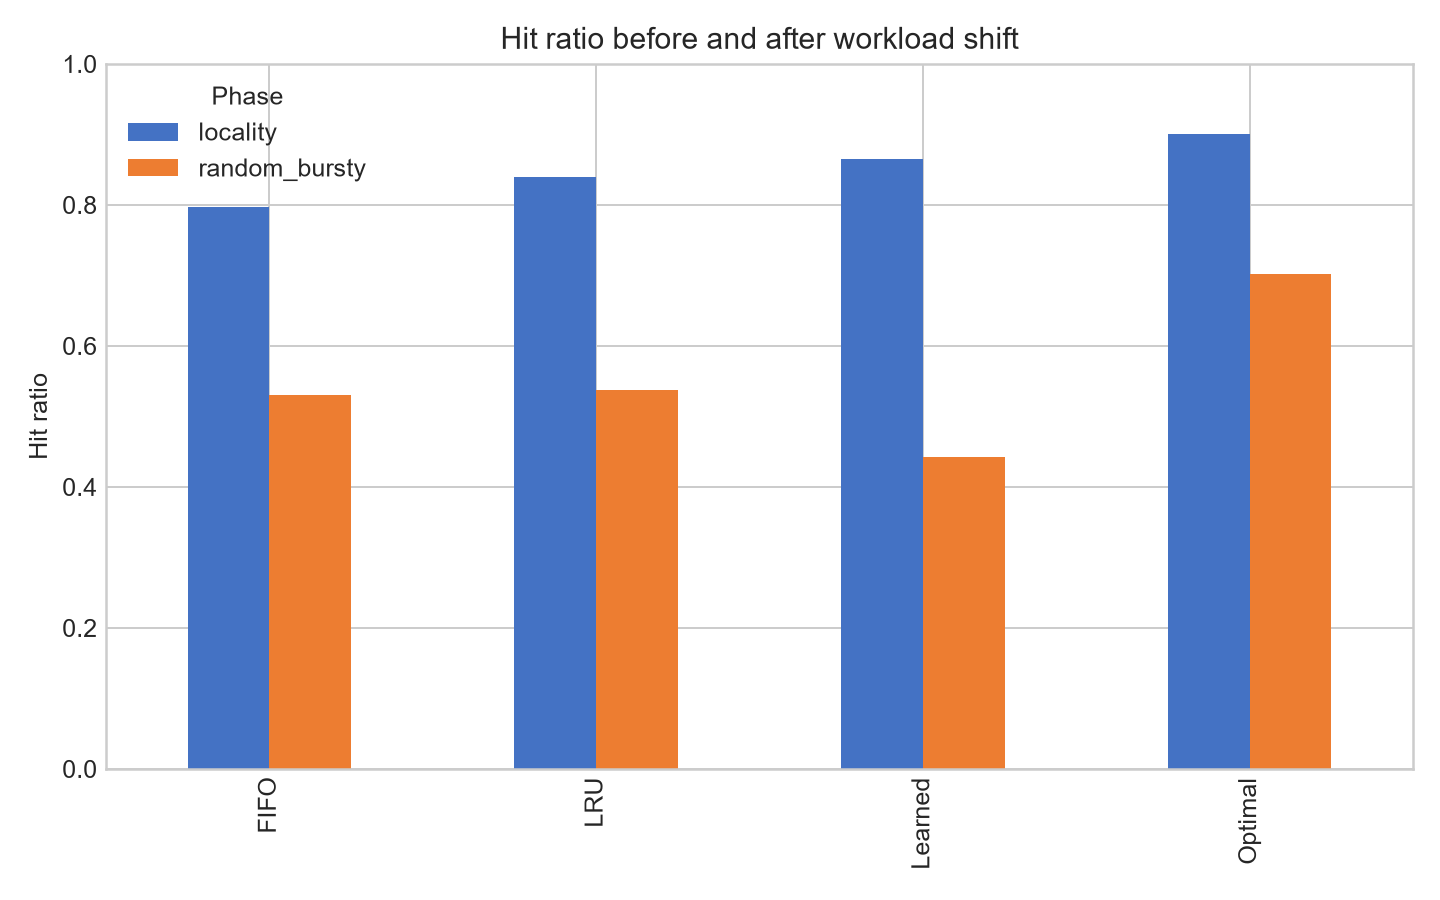
\includegraphics[width=0.82\textwidth]{../results/hit_ratio_by_phase.png}
\caption{Hit ratio before and after the workload shift.}
\end{figure}

\section{Analysis of the Workload Shift}
The workload change hurts all policies because the second phase has a larger active set and less predictable reuse. LRU falls from 84.0\% to 53.8\% hit ratio, while FIFO falls from 79.8\% to 53.0\%. Optimal remains strongest (90.0\% to 70.3\%) because it has future knowledge and therefore shows the best achievable reference point for this trace.

The learned policy reaches 86.5\% in the locality phase, close to Optimal and better than both FIFO and LRU. However, it falls to 44.3\% after the shift, the largest absolute degradation in this experiment. The tree learned relationships from a separate trace whose features were dominated by stable reuse. When the trace becomes random and bursty, age and frequency become less reliable predictors of the next use. This result is useful: learning does not automatically guarantee robustness under drift.

A limitation is that the workload is synthetic and the classifier is intentionally small. A stronger adaptive system could detect phase changes online, retrain periodically, use a larger history window, or combine the learned score with an LRU fallback. Those extensions are outside the base Track 1 scope.

\section{Conclusion}
The classical implementations provide understandable baselines and Optimal supplies an upper bound. The decision tree can improve eviction choices when the workload resembles training conditions, but the shift test shows why operating-system heuristics must be evaluated under distribution change. The main lesson is that a learned component should be monitored and adapted rather than trusted as a permanently correct replacement for a classical policy.

\section*{Reproducibility}
From the repository root, install the packages in \texttt{requirements.txt} and run \texttt{python track1\_page\_replacement.py}. The command regenerates the trace, CSV table, and charts. The existing report can also be generated with \texttt{python generate\_report.py}.

\section*{AI Assistance Disclosure}
An AI coding assistant was used to help structure the implementation, explain standard library APIs, and draft documentation. The workload design, experiment execution, generated measurements, and interpretation should be reviewed and edited by the student before submission.

\end{document}
